\documentclass[11pt]{book}

\usepackage[margin=1in]{geometry}
\usepackage{amsmath,amssymb,amsthm,mathtools}
\usepackage{enumitem}
\usepackage{mathpazo}
\usepackage{xcolor}
\usepackage{tikz}
\usetikzlibrary{arrows.meta,positioning,calc,fit,backgrounds}
\usepackage{mdframed}
\usepackage{booktabs}
\usepackage{tabularx}
\usepackage{hyperref}
\hypersetup{colorlinks=true,linkcolor=blue!50!black,citecolor=blue!50!black,urlcolor=blue!50!black}

% ---------- theorem environments ----------
\theoremstyle{definition}
\newtheorem{definition}{Definition}[section]
\newtheorem{example}[definition]{Example}
\theoremstyle{plain}
\newtheorem{proposition}[definition]{Proposition}
\newtheorem{corollary}[definition]{Corollary}
\newtheorem{theorem}[definition]{Theorem}
\theoremstyle{remark}
\newtheorem{remark}[definition]{Remark}

% ---------- boxes ----------
\newmdenv[
  linecolor=black!70,
  backgroundcolor=black!5,
  linewidth=0.6pt,
  innermargin=10pt,
  outermargin=10pt,
  skipabove=12pt,
  skipbelow=12pt,
  fontcolor=black
]{motto}

\newmdenv[
  linecolor=blue!40!black,
  backgroundcolor=blue!4,
  linewidth=0.6pt,
  innermargin=10pt,
  outermargin=10pt,
  skipabove=12pt,
  skipbelow=12pt
]{reflectionbox}

\newcommand{\ii}{\mathrm{i}}
\newcommand{\hbarcancel}{\hbar}

\title{Variational Principles Compared}
\author{}
\date{}

\begin{document}
\pagestyle{plain}

\chapter{Variational Principles Compared: Hamilton, Maupertuis, Jacobi, Gauss, Hertz, and Schwinger}
\label{ch:variational}

\begin{motto}
\textbf{Motto.} A variational principle is not a single statement but a \emph{family} of statements, distinguished by what is held fixed and what is left free at the endpoints. Hamilton fixes time and lets energy float; Maupertuis fixes energy and lets time float; Gauss and Hertz fix nothing beyond the current instant; Schwinger promotes the whole apparatus to operators. The equations of motion are common ground; the variational scaffolding around them is not.
\end{motto}

\section{Introduction}

Classical mechanics is usually presented as though it had one variational principle: ``the'' principle of least action, $\delta\!\int L\,dt = 0$. In fact the historical record contains a dozen or so logically distinct variational statements about mechanical (and, eventually, quantum) systems, associated with the names of Fermat, Maupertuis, Euler, Hamilton, Jacobi, Gauss, Hertz, Cartan, Weiss, Schwinger, and, in the modern repair of Maupertuis' own principle, Gray, Karl and Novikov. They agree on the trajectories they select in the generic case, which is why they are folded together in most textbook treatments; they disagree, instructively, at exactly the points where the generic case fails --- nonholonomic constraints, free versus fixed transit time, the logical status of momentum, and the passage to quantum mechanics. This chapter lays the principles out side by side, proves the equivalences that hold, and is explicit about the ones that do not.

\begin{table}[h]
\centering
\renewcommand{\arraystretch}{1.25}
\begin{tabular}{@{}ll@{}}
\toprule
Symbol & Meaning \\
\midrule
$q^i,\ \dot q^i$ & generalized coordinates and velocities on configuration space $Q$ \\
$L(q,\dot q,t)$ & Lagrangian \\
$p_i = \partial L/\partial \dot q^i$ & canonical momentum \\
$H(q,p,t)=p_i\dot q^i - L$ & Hamiltonian \\
$S[q(\cdot)]=\int_{t_1}^{t_2} L\,dt$ & Hamilton's action functional \\
$W[q(\cdot)]=\int p_i\,dq^i$ & Maupertuis' abbreviated action \\
$E$ & energy, conserved when $\partial H/\partial t = 0$ \\
$g_{ij}(q)$ & mass (kinetic-energy) metric, $T=\tfrac12 g_{ij}\dot q^i\dot q^j$ \\
$ds_J$ & Jacobi-metric line element, $ds_J^2 = 2(E-V)\,g_{ij}\,dq^i dq^j$ \\
$n(x)$ & refractive index (optics) \\
\bottomrule
\end{tabular}
\caption{Notation used throughout this chapter.}
\end{table}

\section{Preliminaries: the first variation}

\begin{definition}
Let $Q$ be a configuration space and $q:[t_1,t_2]\to Q$ a curve. A \emph{functional} is a map $F$ from curves to $\mathbb{R}$. Given a one-parameter family of curves $q_\varepsilon(t)=q(t)+\varepsilon\,\delta q(t) + O(\varepsilon^2)$ with $\delta q$ vanishing wherever the endpoints are held fixed, the \emph{first variation} is
\[
\delta F := \left.\frac{d}{d\varepsilon}\right|_{\varepsilon=0} F[q_\varepsilon].
\]
A curve is a \emph{stationary point} (extremal) of $F$ if $\delta F=0$ for every admissible $\delta q$.
\end{definition}

For $F[q]=\int_{t_1}^{t_2} L(q,\dot q,t)\,dt$ with fixed endpoints $\delta q(t_1)=\delta q(t_2)=0$, integration by parts gives
\[
\delta S = \int_{t_1}^{t_2}\left(\frac{\partial L}{\partial q^i}-\frac{d}{dt}\frac{\partial L}{\partial \dot q^i}\right)\delta q^i\,dt
\;+\; \left[\frac{\partial L}{\partial \dot q^i}\,\delta q^i\right]_{t_1}^{t_2}.
\]

\begin{remark}
\label{rem:boundary}
The boundary (transversality) term is the whole story of this chapter. Hamilton's principle kills it by fixing $q$ at both ends. Maupertuis' principle keeps the ends of the \emph{curve} fixed but frees the \emph{time} at which they are reached, so a different boundary term survives and has to be handled separately (Section~\ref{sec:maupertuis}). Gauss's and Hertz's principles dispense with the interval altogether and vary only at a single instant (Section~\ref{sec:gauss}). Schwinger's principle promotes the boundary term itself --- $p_i\,\delta q^i$ --- to an operator statement and reads off the canonical commutation relations from it (Section~\ref{sec:schwinger}).
\end{remark}

\section{Hamilton's principle}
\label{sec:hamilton}

\begin{definition}
\textbf{Hamilton's principle.} Among curves $q:[t_1,t_2]\to Q$ with \emph{fixed endpoints in time and configuration}, $q(t_1)=q_1$, $q(t_2)=q_2$, $t_1,t_2$ fixed, the physical trajectory renders the action
\[
S[q(\cdot)] = \int_{t_1}^{t_2} L(q,\dot q,t)\,dt
\]
stationary.
\end{definition}

Setting $\delta S=0$ with the boundary term of the previous section vanishing gives the Euler--Lagrange equations
\[
\frac{d}{dt}\frac{\partial L}{\partial \dot q^i} - \frac{\partial L}{\partial q^i} = 0 .
\]

\begin{remark}[history]
Hamilton's two memoirs, \emph{On a General Method in Dynamics} (1834) and its sequel (1835), are the source of the modern statement, but the underlying calculus-of-variations machinery is Euler's and Lagrange's: Euler's \emph{Methodus inveniendi lineas curvas\ldots} (1744) already extremizes $\int v\,ds$ for a particle under central forces, and Lagrange's \emph{Mécanique analytique} (1788) reorganizes all of mechanics around the Euler--Lagrange equations without yet isolating $\int L\,dt$ as the object being varied. Hamilton arrived at the dynamical principle from the optical side: his earlier work on the \emph{characteristic function} in geometrical optics (1824--1832) is formally the same variational structure applied to light rays, and he treats mechanics and optics as two instances of one theory throughout the 1834 memoir.
\end{remark}

\begin{remark}[fragility]
\label{rem:fragility}
Hamilton's principle, applied without further thought to a system with \emph{nonholonomic} velocity constraints $a^{(k)}_i(q)\dot q^i=0$ by adjoining the constraints to $L$ with Lagrange multipliers before varying, produces the \emph{vakonomic} equations of motion. These generically disagree with the correct Lagrange--d'Alembert equations for a nonholonomically constrained system (the textbook example is a coin or sphere rolling without slipping). The discrepancy is not a paradox to be explained away: it is a sign that Hamilton's principle, in its integral, fixed-endpoint form, is simply not the right variational statement for a constraint that is imposed at the level of velocities rather than configurations. Section~\ref{sec:gauss} shows which principle \emph{is} the right one.
\end{remark}

\section{Maupertuis' principle}
\label{sec:maupertuis}

\begin{definition}
\label{def:maupertuis-old}
\textbf{Maupertuis' principle (principle of least action, abbreviated form).} Suppose $H$ has no explicit time dependence, so $E=H$ is conserved. Among curves in configuration space joining $q_1$ to $q_2$ that are compatible with energy $E$ --- with the \emph{time of transit left free} --- the physical trajectory renders the abbreviated action
\[
W[q(\cdot)] = \int p_i\,dq^i
\]
stationary, where along each trial curve $p_i$ is fixed pointwise by the energy constraint $H(q,p)=E$.
\end{definition}

\begin{remark}[history and priority]
Maupertuis announced a least-action principle for the refraction of light in 1744 (\emph{Accord de différentes lois de la nature qui avaient jusqu'ici paru incompatibles}), arguing that nature economizes a quantity of ``action'' distinct from Fermat's time, and generalized it to mechanics at large in 1746 (\emph{Les loix du mouvement et du repos déduites d'un principe métaphysique}). The generalization was, however, put into usable mathematical form not by Maupertuis but by Euler, whose 1744 \emph{Additamentum II} already shows that $\int v\,ds$ is stationary along the true trajectory of a particle under a central force --- a priority dispute (sharpened by Samuel König's accusation of plagiarism and Voltaire's public mockery of Maupertuis) that is one of the uglier episodes in eighteenth-century science but does not affect the mathematics.
\end{remark}

\begin{remark}[Jacobi's complaint]
\label{rem:jacobi-complaint}
Definition~\ref{def:maupertuis-old} constrains the energy \emph{pointwise} on every trial curve, $H(q,p)=E$, not merely on the true trajectory. Jacobi himself objected, in the \emph{Vorlesungen über Dynamik}, that the principle is presented in essentially every textbook so as to be nearly unintelligible, and the pointwise constraint is the reason why: it presupposes on trial curves the very energy conservation that Hamilton's principle only \emph{derives} for the true one, and in low dimension it leaves almost nothing left to vary (fixing $E=v^2/2$ for a free particle on a line, for instance, fixes the speed outright). Section~\ref{sec:reciprocal} gives the repaired version, due to Gray, Karl and Novikov, in which only the trial curve's \emph{mean} energy is held fixed.
\end{remark}

\begin{proposition}
\label{prop:S-W}
On a trajectory of constant energy $E$,
\[
S[q(\cdot)] = W[q(\cdot)] - E\,(t_2-t_1).
\]
\end{proposition}
\begin{proof}
$L = p_i\dot q^i - H = p_i\dot q^i - E$ along such a trajectory, so
\[
S=\int_{t_1}^{t_2}\!\big(p_i\dot q^i-E\big)\,dt=\int_{t_1}^{t_2}\! p_i\dot q^i\,dt \;-\;E(t_2-t_1)=\int_{q_1}^{q_2}\! p_i\,dq^i-E(t_2-t_1)=W-E(t_2-t_1). \qedhere
\]
\end{proof}

\begin{theorem}[equivalence, isoenergetic case]
Among curves of fixed energy $E$ joining $q_1$ to $q_2$, with transit time free, $\delta W=0$ if and only if the curve, traversed according to $H=E$, satisfies Hamilton's equations.
\end{theorem}
\begin{proof}[Proof sketch]
Vary $S=W-E\Delta t$ under the enlarged class of variations that also displace the final time by $\delta t_2$, holding $E$ fixed on the varied curves (an isoenergetic variation). The extra boundary contribution from freeing $t_2$ is $\left(L - p_i\dot q^i\right)\delta t_2=-E\,\delta t_2$, which exactly cancels the corresponding term coming from $\delta(E\Delta t)$ under the constraint $\delta E=0$. What remains is $\delta W=0$ subject to the fixed-energy constraint, with no leftover boundary term --- i.e. the same Euler--Lagrange content as Hamilton's principle, now expressed with time eliminated in favor of $E$. A fully rigorous treatment of this constrained (isoperimetric-type) variational problem is given in Whittaker, \emph{Analytical Dynamics}, \S99, and Lanczos, \emph{The Variational Principles of Mechanics}, ch.~5. As Remark~\ref{rem:jacobi-complaint} flags, this argument only handles trial curves that already conserve $E$ pointwise; Section~\ref{sec:reciprocal} removes that restriction.
\end{proof}

\begin{remark}
$W$ and $S$ therefore extremize over \emph{different} classes of curves and are not interchangeable term by term: $S$'s stationarity theorem fixes the parametrization (time) and lets energy be whatever it turns out to be; $W$'s fixes the energy and is blind to parametrization, recovering only the trajectory as a set of points in $Q$ (the orbit shape), with the time-parametrization reconstructed afterward from $H=E$. This is why Maupertuis' principle is the natural one for questions about orbit \emph{shape} (is the Kepler orbit closed? what is its precession?) while Hamilton's is the natural one for questions about time evolution.
\end{remark}

\section{Reciprocal principles and the generalized Maupertuis principle}
\label{sec:reciprocal}

Gray, Karl and Novikov repaired Maupertuis' principle by weakening the pointwise energy constraint of Definition~\ref{def:maupertuis-old} to a constraint on the trial curve's \emph{time-averaged} energy alone --- a constraint every trial curve can satisfy, and one that no longer presupposes what Hamilton's principle is supposed to derive.

\begin{definition}
For a trial trajectory $q(\cdot)$ of duration $T=t_2-t_1$ joining fixed $q_1,q_2$, the \emph{mean energy} is
\[
\bar E := \frac1T\int_{t_1}^{t_2} H(q,p,t)\,dt .
\]
On the true trajectory of a conservative system $\bar E=E$, but on an arbitrary trial curve $\bar E$ is perfectly well defined even when $H$ is not pointwise constant along it.
\end{definition}

\begin{definition}
\textbf{The Generalized Maupertuis Principle (GMP).} Among trial curves with fixed endpoints $q_1,q_2$ and fixed \emph{mean} energy $\bar E$, transit time $T$ left free, the true trajectory renders $W=\int p_i\,dq^i$ stationary:
\[
(\delta W)_{\bar E} = 0 .
\]
\end{definition}

\begin{proposition}[generalization of Proposition~\ref{prop:S-W}]
For \emph{any} trial trajectory, not only one of constant energy,
\[
\bar E\,T = W - S .
\]
\end{proposition}
\begin{proof}
Identical to the proof of Proposition~\ref{prop:S-W}, with $E$ replaced by $\bar E=\frac1T\int H\,dt$ throughout: $S=\int(p_i\dot q^i - H)\,dt = W - \bar E T$.
\end{proof}

Varying this identity at fixed endpoints, with both the trial curve and the duration $T$ free, splits into two independent statements (Gray--Karl--Novikov, \S2.2): fixing $T$ recovers Hamilton's principle $(\delta S)_T=0$; fixing $\bar E$ instead gives the GMP $(\delta W)_{\bar E}=0$. The two are therefore equivalent to each other, and --- unlike the textbook Maupertuis principle of Definition~\ref{def:maupertuis-old} --- the GMP derives energy conservation for the true trajectory rather than assuming it, resolving Jacobi's complaint.

\begin{definition}
Reversing which quantity is held fixed and which is left free in each principle gives its \emph{reciprocal}: the \textbf{Reciprocal Maupertuis Principle (RMP)},
\[
(\delta \bar E)_W = 0,
\]
and the \textbf{Reciprocal Hamilton Principle (RHP)},
\[
(\delta T)_S = 0 .
\]
The RMP is a principle of \emph{least (stationary) mean energy} at fixed action $W$; the RHP is a principle of \emph{least time} at fixed action $S$.
\end{definition}

\begin{theorem}[the reciprocity--Legendre square]
The four statements $(\delta \bar E)_W=0$, $(\delta W)_{\bar E}=0$, $(\delta S)_T=0$, and $(\delta T)_S=0$ are pairwise equivalent (each characterizes the same true trajectories): horizontal neighbors in Figure~\ref{fig:square} are related by \emph{reciprocity} (swapping which member of a conjugate pair is fixed and which is varied), and vertical neighbors by the \emph{Legendre} relation $\bar ET=W-S$.
\end{theorem}

\begin{figure}[h]
\centering
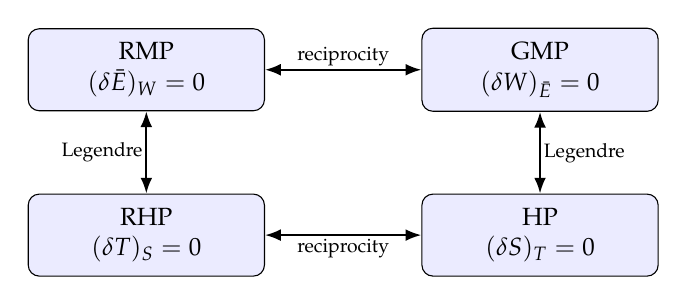
\begin{tikzpicture}[
  box/.style={draw, rounded corners, align=center, minimum height=8mm, minimum width=30mm, inner sep=5pt, font=\small},
  arr/.style={thick, {Latex[length=2mm]}-{Latex[length=2mm]}},
  lbl/.style={font=\scriptsize, fill=white, inner sep=1pt}
]
  \node[box, fill=blue!8] (rmp) at (0,2.1) {RMP\\ $(\delta \bar E)_W=0$};
  \node[box, fill=blue!8] (gmp) at (5,2.1) {GMP\\ $(\delta W)_{\bar E}=0$};
  \node[box, fill=blue!8] (rhp) at (0,0) {RHP\\ $(\delta T)_S=0$};
  \node[box, fill=blue!8] (hp) at (5,0) {HP\\ $(\delta S)_T=0$};
  \draw[arr] (rmp) -- node[lbl,above]{reciprocity} (gmp);
  \draw[arr] (rhp) -- node[lbl,below]{reciprocity} (hp);
  \draw[arr] (rmp) -- node[lbl,left]{Legendre} (rhp);
  \draw[arr] (gmp) -- node[lbl,right]{Legendre} (hp);
\end{tikzpicture}
\caption{The reciprocity--Legendre square of Gray, Karl and Novikov. Horizontal arrows swap what is held fixed and what is varied; vertical arrows exchange $(W,\bar E)$ for $(S,T)$ via $\bar ET=W-S$.}
\label{fig:square}
\end{figure}

\begin{remark}[RMP as the classical limit of Rayleigh--Ritz]
For periodic, quasiperiodic or otherwise steady-state motion, the RMP is the $\hbar\to0$ limit of the Schrödinger variational principle $(\delta\langle\hat H\rangle)_n=0$ of quantum mechanics: for large quantum number $n$, $\langle\hat H\rangle$ becomes the classical mean energy and $n$ becomes proportional to the classical action $W$ over a cycle (Karl and Novikov). This makes the RMP the natural tool for semiclassical (EBK/torus) quantization, exactly as the ordinary Rayleigh--Ritz method is the natural tool for estimating quantum energy levels from trial wavefunctions; for periodic and quasiperiodic motion it further coincides with Percival's variational principle for invariant tori.
\end{remark}

\section{Jacobi's principle: geometrization}
\label{sec:jacobi}

For a natural system, $T=\tfrac12 g_{ij}(q)\dot q^i\dot q^j$ defines a Riemannian metric $g_{ij}$ on $Q$ (the mass metric), and $p_i\,dq^i = g_{ij}\dot q^j\,dq^i = 2T\,dt$ along any trajectory. Writing $ds^2=g_{ij}\,dq^idq^j$ for the mass-metric line element, $dt = ds/\sqrt{2T}=ds/\sqrt{2(E-V)}$, so
\[
W=\int 2(E-V)\,dt = \int \sqrt{2(E-V)}\;ds .
\]

\begin{definition}
\label{def:jacobi-metric}
The \emph{Jacobi metric} is the conformal rescaling
\[
ds_J^2 := 2\big(E-V(q)\big)\,g_{ij}(q)\,dq^i\,dq^j,
\]
defined on the region $\{E>V\}$ where motion is classically allowed.
\end{definition}

\begin{corollary}
Maupertuis' principle is exactly the statement that trajectories of energy $E$ are \emph{geodesics} of the Jacobi metric: $\delta\!\int ds_J = 0$.
\end{corollary}

This is Jacobi's reformulation (\emph{Vorlesungen über Dynamik}, lectures of 1842--43, published posthumously in 1866 by Clebsch): dynamics at fixed energy is pure Riemannian geometry, with the potential absorbed into the metric. Two consequences are worth flagging because they recur elsewhere in this book: (i) the curvature of $g^J_{ij}=2(E-V)g_{ij}$ controls the stability of nearby trajectories exactly as sectional curvature controls geodesic deviation, giving a direct route from a potential $V(q)$ to exponential trajectory divergence (Krylov's original argument for mixing in the hard-sphere gas, later formalized for Anosov geodesic flows); (ii) since $Q$ and its metric are usually finite-dimensional and time has been eliminated entirely, the Jacobi picture is the cleanest illustration that ``geometrize first, quantize/perturb second'' is a genuine choice of route, not a cosmetic rewriting.

\section{A genuine non-equivalence: multi-well potentials and brake orbits}
\label{sec:nonequivalence}

Every equivalence proved so far --- Proposition~\ref{prop:S-W}, the isoenergetic theorem, the reciprocity--Legendre square of Section~\ref{sec:reciprocal} --- is \emph{local}: each relates a single given trajectory to itself, under different fixed/free bookkeeping. None of them says that the \emph{set} of trajectories obtained by prescribing $T$ in advance (Hamilton) coincides with the set obtained by prescribing $E$ in advance (Maupertuis/GMP). Once the potential has more than one local minimum, these two sets --- and even their cardinalities --- generically differ.

\begin{remark}[trial curves live in different domains]
Hamilton's principle imposes no restriction on trial curves at all: $q(t)$ may pass through any point of $Q$, at any speed, en route from $q_1$ to $q_2$, since $L=T(\dot q)-V(q)$ is perfectly well defined however fast or slow a trial curve moves at a given $q$. The textbook Maupertuis principle (Definition~\ref{def:maupertuis-old}) is different in kind: $p$ along the trial curve is \emph{defined} by $H(q,p)=E$, so $T=E-V(q)$ must be $\ge0$ pointwise --- a trial curve can only exist within the classically allowed (Hill's) region $Q_E:=\{q\in Q: V(q)\le E\}$, exactly the domain restriction already flagged in the Jacobi metric of Definition~\ref{def:jacobi-metric}. If $q_1$ and $q_2$ lie in different path-components of $Q_E$ --- separated by a barrier taller than $E$ --- the textbook Maupertuis competition at that $E$ has no trial curves joining them at all, not merely no minimizer. The GMP of Section~\ref{sec:reciprocal} repairs this too: since only the \emph{mean} energy is fixed, a GMP trial curve is exactly as free as a Hamilton one, dipping in and out of $\{V>E\}$ as it pleases, provided the time-average works out to $\bar E$. But this freedom is only in the trial family: the actual extremal, once found, is a genuine solution of an autonomous Hamiltonian system and so has \emph{constant} energy equal to its own mean. If that constant falls below a barrier separating $q_1$ from $q_2$, no connecting extremal exists in the GMP formulation any more than in Hamilton's --- not because of how the competition was set up, but because ordinary energy conservation forbids it.
\end{remark}

\begin{remark}[multiplicity: Seifert's brake orbits]
Even granting accessibility, the \emph{number} of genuine trajectories connecting two points at one fixed $E$ need not match the number connecting them in one fixed $T$. Let $\Omega_E:=\{q:V(q)\le E\}$ be a bounded potential well with $E$ a regular value of $V$. Via the Jacobi metric, a trajectory that oscillates back and forth within $\Omega_E$ --- a \emph{brake orbit}, so called because the particle momentarily comes to rest, $p=0$, at each end of its swing, on $\partial\Omega_E$ --- corresponds exactly to a geodesic chord of $ds_J$ meeting $\partial\Omega_E$ orthogonally. Seifert (1948) proved that at least one such orbit always exists, and conjectured at least $N=\dim Q$ geometrically distinct ones whenever $\Omega_E$ is homeomorphic to an $N$-disk: genuine multiplicity of fixed-energy solutions, expected already in a single, topologically trivial well, before a second minimum is ever introduced. The conjecture is now a theorem under a concavity hypothesis on $\partial\Omega_E$ (Giambò, Giannoni and Piccione), and is known to fail without some such hypothesis: the same authors exhibit real-analytic wells, homeomorphic to a disk, carrying only \emph{one} brake orbit. None of this multiplicity is visible from the Hamilton side by fixing a single $T$ and solving once: each brake orbit has its own period, generically different from the others, so a fixed-$T$ search catches at most whichever one happens to match.
\end{remark}

\begin{remark}[what survives]
None of this contradicts Section~\ref{sec:reciprocal}: trajectory by trajectory, Hamilton's and Maupertuis'/GMP's principles remain exactly equivalent. What fails is the stronger, unstated assumption that fixing $T$ and fixing $E$ pose ``the same problem'' with the same solution count. Once $\Omega_E$ has nontrivial topology --- exactly what a potential with several minima produces, once $E$ rises above the barriers separating them --- fixing $E$ and fixing $T$ become genuinely different slicings of one underlying family of solutions: governed, on the Maupertuis side, by the topology of $\Omega_E$ (Seifert, Ljusternik--Schnirelmann category); and, on the Hamilton side, by a related but distinct Morse theory of the fixed-time path space. ``Maupertuis' principle is equivalent to Hamilton's principle'' is therefore true of individual trajectories, and false, in general, of the two boundary-value \emph{problems}.
\end{remark}

\section{Fermat's principle: the optical model}
\label{sec:fermat}

\begin{definition}
\textbf{Fermat's principle} (1662). A light ray joining two points extremizes the optical path length $\int n(x)\,ds$, where $n$ is the refractive index and $ds$ is Euclidean arc length.
\end{definition}

The analogy that Maupertuis and Euler exploited, and that Hamilton later made structurally precise, is
\[
\text{optics:}\ \ \delta\!\int n(x)\,ds = 0
\qquad\longleftrightarrow\qquad
\text{mechanics:}\ \ \delta\!\int \sqrt{2(E-V)}\,ds = 0,
\]
i.e. $n(x)\leftrightarrow\sqrt{2(E-V(x))}$: a mechanical particle refracts at a potential step exactly as a light ray refracts at an interface, with ``optical density'' standing in for ``local speed at fixed energy.'' This is not merely decorative. Hamilton's own route to dynamics went through his earlier optical work; the same analogy, run in the other direction, is what motivated the eikonal (geometrical-optics) limit of wave optics and, via de Broglie and Schrödinger, the $\hbar\to0$ correspondence between the Schrödinger equation and Hamilton--Jacobi theory. It is one of the few places in physics where a nineteenth-century analogy was later upgraded to an exact singular limit ($\hbar\to0$) rather than discarded once its origin was understood.

\section{Gauss's principle of least constraint}
\label{sec:gauss}

Hamilton's and Maupertuis' principles are \emph{integral} statements: they compare an entire trial curve against neighboring curves over a finite stretch of time or a finite arc. Gauss's principle (1829, \emph{Über ein neues allgemeines Grundgesetz der Mechanik}) is of a different logical kind: it is \emph{differential}, comparing only candidate accelerations at the current instant.

\begin{definition}
\textbf{Gauss's principle of least constraint.} For particles of mass $m_a$ at given positions and velocities, subject to (possibly nonholonomic) constraints, and acted on by applied forces $\vec F_a$, the true accelerations $\ddot{\vec r}_a$ minimize
\[
Z(\ddot{\vec r}) := \sum_a m_a\left|\ddot{\vec r}_a - \frac{\vec F_a}{m_a}\right|^2
\]
over all accelerations compatible with the constraints differentiated to the acceleration level, positions and velocities held fixed.
\end{definition}

\begin{proposition}
\label{prop:gauss-dalembert}
Gauss's principle is equivalent to d'Alembert's principle (and hence to Newton's second law together with the constraint forces doing no virtual work).
\end{proposition}
\begin{proof}[Proof sketch]
Minimizing the quadratic form $Z$ over the affine space of admissible $\ddot{\vec r}_a$ sets its gradient orthogonal (in the mass inner product) to the tangent space of admissible \emph{variations} $\delta\ddot{\vec r}_a$ of that space, i.e.
\[
\sum_a \big(m_a\ddot{\vec r}_a - \vec F_a\big)\cdot \delta\ddot{\vec r}_a = 0
\]
for every admissible $\delta \ddot{\vec r}_a$. For the constraints in question, admissible acceleration-variations and admissible virtual displacements $\delta \vec r_a$ span the same subspace, so this is exactly d'Alembert's principle, $\sum_a(m_a\ddot{\vec r}_a-\vec F_a)\cdot\delta\vec r_a=0$.
\end{proof}

\begin{remark}[resolving Section~\ref{sec:hamilton}]
Because Gauss's principle is imposed directly on the constraint manifold at the acceleration level, it reproduces the Lagrange--d'Alembert equations for a nonholonomic system \emph{by construction}, with no vakonomic detour. The mismatch flagged in Section~\ref{sec:hamilton} is therefore not a defect in mechanics but a mismatch of variational \emph{principles} to the constraint type: integral, fixed-endpoint principles (Hamilton, Maupertuis) are suited to holonomic constraints; the differential, instantaneous principle (Gauss) handles nonholonomic ones correctly because it never has to compare curves that end differently far along a constraint surface that the constraint itself does not let you parametrize by position alone.
\end{remark}

\begin{remark}[Gibbs--Appell form]
Gauss's principle is usually stated in physical acceleration variables, but it restates without loss in terms of \emph{quasi-accelerations} $\dot\omega^r$ adapted to the constraints: minimizing $Z$ over admissible quasi-accelerations gives the \emph{Gibbs--Appell equations} $\partial\mathcal S/\partial\dot\omega^r = Q_r$, where $\mathcal S:=\tfrac12\sum_a m_a|\ddot{\vec r}_a|^2$ --- the same quantity Gauss minimizes, re-expressed --- is the \emph{Gibbs function} and $Q_r$ are the generalized forces conjugate to the quasi-velocities. Gibbs (1879) and, independently, Appell (1900) introduced this form because it handles constraints of arbitrarily general type, even nonlinear in the velocities, without ever introducing a Lagrange multiplier --- a second, independent route to the resolution Remark~\ref{rem:fragility} promised.
\end{remark}

\section{Hertz's principle of least curvature}
\label{sec:hertz}

\begin{definition}
\textbf{Hertz's principle} (\emph{Die Prinzipien der Mechanik}, 1894). A system subject only to holonomic (``rigid'') constraints and no applied forces moves, at constant speed, along the path of \emph{least curvature} through configuration space equipped with the mass metric $g_{ij}$.
\end{definition}

\begin{corollary}
Hertz's principle is the $V\equiv 0$ specialization of Jacobi's principle.
\end{corollary}
\begin{proof}
Set $V=0$ in the Jacobi metric: $ds_J^2 = 2E\,g_{ij}\,dq^idq^j$, a \emph{constant} conformal rescaling of $g_{ij}$. Geodesics are unchanged by a constant conformal factor (only their affine speed changes, to $\sqrt{2E}$), so the $ds_J$-geodesics coincide with the $g_{ij}$-geodesics, traversed at constant speed. ``Least curvature'' is Hertz's own (equivalent) way of characterizing a geodesic: the path whose curvature vector, computed in $g_{ij}$, vanishes.
\end{proof}

This is precisely the ``forceless mechanics'' discussed elsewhere in this book: what looks like force-free inertial motion in a curved configuration space (e.g.\ a bead constrained to a curved wire, or the reduced dynamics of a system with cyclic coordinates eliminated) is literally geodesic motion once the constraints have been folded into the metric $g_{ij}$ --- Hertz's proposal to eliminate force from the foundations of mechanics amounts to insisting that \emph{all} of dynamics should look like this, with potentials themselves eventually explained away via hidden constrained (``cyclic'') degrees of freedom.

\section{Herglotz's principle: a genuine variational principle for dissipation}
\label{sec:herglotz}

Every principle so far --- Hamilton's, Maupertuis'/GMP's, Jacobi's, Gauss's, Hertz's --- governs conservative, or at worst constrained-but-reversible, systems: none of them, as stated, can produce a genuinely dissipative equation of motion, one along which mechanical energy is not conserved. The usual patch, Rayleigh's dissipation function added by hand to the Euler--Lagrange equations, is exactly that: a patch, not the output of extremizing any single functional. Herglotz's principle removes the patch.

\begin{definition}
\textbf{Herglotz's variational principle} (1930). Let $L(q,\dot q,z,t)$ depend on an auxiliary variable $z$ as well as on $q,\dot q,t$, and let $z(\cdot)$ be determined along any trial curve $q(\cdot)$ by
\[
\dot z(t) = L\big(q(t),\dot q(t), z(t), t\big), \qquad z(t_1)=z_1 \text{ fixed}.
\]
The true trajectory renders the \emph{endpoint value} $z(t_2)$ stationary among curves with fixed $q(t_1)=q_1$, $q(t_2)=q_2$: $\delta z(t_2) = 0$.
\end{definition}

\begin{remark}
When $L$ does not depend on $z$, $z(t_2)-z_1=\int_{t_1}^{t_2}L\,dt$ and Herglotz's principle reduces to Hamilton's. The dependence on $z$ is the whole extension.
\end{remark}

\begin{proposition}
Herglotz's principle is equivalent to the generalized Euler--Lagrange equations
\[
\frac{d}{dt}\frac{\partial L}{\partial\dot q^i} - \frac{\partial L}{\partial q^i} - \frac{\partial L}{\partial z}\frac{\partial L}{\partial\dot q^i} = 0 .
\]
\end{proposition}
\begin{proof}
Linearize the defining ODE along a variation $\delta q^i$ (with $\delta q^i(t_1)=\delta q^i(t_2)=0$, hence $\delta z(t_1)=0$): $\delta\dot z = \frac{\partial L}{\partial q^i}\delta q^i+\frac{\partial L}{\partial \dot q^i}\delta\dot q^i+\frac{\partial L}{\partial z}\delta z$, a linear ODE for $\delta z$ along the trajectory. With the integrating factor $\mu(t):=\exp\!\big(-\int_{t_1}^t \frac{\partial L}{\partial z}\,dt'\big)$, so $\dot\mu=-\mu\,\partial L/\partial z$, this becomes $\frac{d}{dt}(\mu\,\delta z) = \mu\left(\frac{\partial L}{\partial q^i}\delta q^i+\frac{\partial L}{\partial\dot q^i}\delta\dot q^i\right)$. Integrating from $t_1$ to $t_2$ and integrating the $\delta\dot q^i$ term by parts (the boundary contribution vanishes since $\delta q^i(t_1)=\delta q^i(t_2)=0$, and $\frac{d}{dt}\big(\mu\,\partial L/\partial\dot q^i\big)=\mu\big(\frac{d}{dt}\frac{\partial L}{\partial\dot q^i}-\frac{\partial L}{\partial z}\frac{\partial L}{\partial\dot q^i}\big)$ since $\dot\mu/\mu=-\partial L/\partial z$) gives
\[
\mu(t_2)\,\delta z(t_2) = \int_{t_1}^{t_2}\mu\left[\frac{\partial L}{\partial q^i}-\frac{d}{dt}\frac{\partial L}{\partial\dot q^i}+\frac{\partial L}{\partial z}\frac{\partial L}{\partial \dot q^i}\right]\delta q^i\,dt .
\]
Since $\mu(t_2)\neq0$, $\delta z(t_2)=0$ for every admissible $\delta q^i$ forces the bracket to vanish.
\end{proof}

\begin{example}
Take $L=\tfrac12 m\dot q^2 - V(q) - \gamma z$ for constant $\gamma$. Then $\partial L/\partial z=-\gamma$, and the generalized Euler--Lagrange equation reads
\[
m\ddot q + V'(q) + \gamma m\dot q = 0,
\]
the ordinary linearly-damped equation of motion --- genuine viscous friction, obtained from the stationarity of a single functional, with no dissipation function added by hand. This is exactly the kind of open-system equation discussed elsewhere in this book (Meshchersky, Bateman's dual Lagrangian, Abraham--Lorentz); Herglotz's principle is the general variational scaffold those examples are individual instances of.
\end{example}

Herglotz gave this construction in unpublished 1930 Göttingen lectures; it re-entered the literature only via Georgieva and Guenther's rediscovery (2002), and a decade later Bravetti, Cruz and Tapias recognized it as the variational principle native to \emph{contact}, rather than symplectic, geometry --- the natural geometric home for dissipative mechanics, exactly as symplectic geometry is the natural home for the conservative principles of Sections~\ref{sec:hamilton}--\ref{sec:hertz}. This is a second illustration of Section~\ref{sec:primacy}'s thesis, running in the opposite direction from Remark~\ref{rem:fragility}: friction was never in doubt as physics, and it took decades to notice that a single genuine variational principle --- not a patched-on dissipation function --- could be engineered to produce it.

\section{Schwinger's action principles: classical and quantum}
\label{sec:schwinger}

\subsection{The classical phase-space principle}
\label{sec:schwinger-classical}

Every principle so far, once phase space is introduced, treats $p_i$ as \emph{derived}: $p_i:=\partial L/\partial\dot q^i$, fixed in terms of $q,\dot q$ before any variation is taken. There is an older and logically different construction, due to Cartan (1922) and extended to field theory by Weiss (1936, 1938), in which $q^i(t)$ and $p_i(t)$ are varied as \emph{independent} functions, with no relation between them assumed in advance. Schwinger opens his 1951 paper on this classical construction before promoting it to operators.

\begin{definition}
\textbf{The classical phase-space action principle (Cartan--Weiss--Schwinger).} Let $q^i(t)$ and $p_i(t)$ be independent trial functions on $[t_1,t_2]$, and define
\[
\tilde S[q(\cdot),p(\cdot)] := \int_{t_1}^{t_2}\big(p_i\dot q^i - H(q,p,t)\big)\,dt .
\]
The true motion renders $\tilde S$ stationary under independent variations $\delta q^i$ (vanishing at $t_1,t_2$) and $\delta p_i$ (unconstrained at the endpoints, since $p$ appears undifferentiated).
\end{definition}

\begin{proposition}
Independent stationarity in $\delta p_i$ and $\delta q^i$ yields, separately,
\[
\dot q^i = \frac{\partial H}{\partial p_i}
\qquad\text{and}\qquad
\dot p_i = -\frac{\partial H}{\partial q^i},
\]
i.e.\ \emph{both} of Hamilton's equations, with no leftover boundary term beyond $\big[p_i\,\delta q^i\big]_{t_1}^{t_2}$.
\end{proposition}
\begin{proof}
\[
\delta\tilde S = \int_{t_1}^{t_2}\left[\left(\dot q^i - \frac{\partial H}{\partial p_i}\right)\delta p_i - \left(\dot p_i + \frac{\partial H}{\partial q^i}\right)\delta q^i\right]dt + \big[p_i\,\delta q^i\big]_{t_1}^{t_2},
\]
obtained by integrating the $p_i\delta\dot q^i$ term by parts. Since $\delta p_i$ and $\delta q^i$ are independent and unconstrained in the interior, the two bracketed coefficients must vanish separately, and $\delta q^i(t_1)=\delta q^i(t_2)=0$ kills the boundary term.
\end{proof}

\begin{remark}
This is a different logical achievement from Hamilton's principle of Section~\ref{sec:hamilton}. There, only $q$ is varied and $p:=\partial L/\partial\dot q$ is a definition, so only the second Hamilton equation is derived --- the first is built into the definition of $p$ before variation ever starts. Here neither equation is assumed: treating $q$ and $p$ as coordinates of equal standing on phase space, with no a priori link between $p$ and $\dot q$, derives \emph{both} canonical equations symmetrically. It is exactly this symmetry between $q$ and $p$ --- and the resulting boundary term $p_i\,\delta q^i$, free of any assumed relation between the two --- that Schwinger promotes to an operator statement next.
\end{remark}

\subsection{Promotion to the quantum action principle}
\label{sec:schwinger-quantum}

Schwinger's action principle (1951, \emph{The Theory of Quantized Fields I}) extends the classical phase-space principle of Section~\ref{sec:schwinger-classical} to quantum transition amplitudes, and does so differentially rather than by summing over trial histories.

\begin{definition}
\textbf{Schwinger's quantum action principle.} Let $S$ be the action operator, a functional of the Heisenberg-picture dynamical variables between times $t_1$ and $t_2$. For an arbitrary infinitesimal variation $\delta$ --- of the Lagrangian, of the dynamical variables, or of the boundary configurations/times themselves ---
\[
\delta \langle q_2 t_2 \,|\, q_1 t_1\rangle = \frac{\ii}{\hbar}\,\langle q_2 t_2\,|\,\delta S\,|\,q_1 t_1\rangle .
\]
\end{definition}

Three distinct classical statements are packed into this one operator statement, depending on what is varied:
\begin{enumerate}[label=(\roman*)]
\item Varying the trajectory operators with fixed boundary configurations and demanding the matrix element be stationary yields the \emph{operator} Euler--Lagrange (Heisenberg) equations of motion --- the operator counterpart of Section~\ref{sec:hamilton}.
\item Varying only the endpoint configuration $q_2$ produces a surviving boundary term $\tfrac{\ii}{\hbar}\langle q_2t_2|\,p_i\,\delta q^i\,|q_1t_1\rangle$ --- the direct operator promotion of the boundary term $p_i\,\delta q^i$ isolated in Section~\ref{sec:schwinger-classical}, where $q$ and $p$ were already independent. Requiring this to be realizable consistently as an operator relation --- i.e.\ that $p_i$ generate translations of $q^i$ the way a momentum should --- is how Schwinger arrives at the canonical commutation relations $[q^i,p_j]=\ii\hbar\,\delta^i_j$ from the action principle, rather than postulating them independently of the dynamics as in canonical quantization. This step would not be available starting from ordinary Hamilton's principle, where $p$ is only ever a derived shorthand for $\partial L/\partial\dot q$ and never an independent operator waiting to be assigned a commutator.
\item In the regime where the phase $S/\hbar$ varies rapidly compared to $\hbar$ itself (formally $\hbar\to0$), the matrix element is dominated by the classical trajectory of extremal $S$, and (i) reduces to ordinary Hamilton's principle.
\end{enumerate}

\begin{remark}[Schwinger versus Feynman]
Feynman's 1948 path-integral formulation (\emph{Space-Time Approach to Non-Relativistic Quantum Mechanics}) expresses the same transition amplitude as a genuine sum over \emph{all} paths, most of which do not satisfy any classical equation of motion, weighted by $e^{\ii S[q]/\hbar}$:
\[
\langle q_2t_2|q_1t_1\rangle = \int \mathcal D[q(\cdot)]\;e^{\ii S[q]/\hbar}.
\]
Classical Hamilton's principle re-emerges from this integral principle by stationary phase as $\hbar\to0$: paths away from the classical trajectory interfere destructively. Schwinger's principle, by contrast, never introduces off-shell paths at all; it is a \emph{differential} statement about how the amplitude responds to a variation, applied directly to operators that already satisfy their equations of motion. The two are provably equivalent as calculational tools, but they generalize least-action reasoning along different axes: Feynman's toward a probabilistic/interference statement, Schwinger's toward an algebraic, operator statement closer in spirit to Gauss's and Hertz's differential principles than to Hamilton's integral one --- despite Schwinger's action $S$ itself being, like Hamilton's, a time integral. (This hybrid character --- differential in what is varied, integral in what is being varied \emph{of} --- is genuinely a different species from Gauss's principle and should not be flattened into the same row of any classification table; see Section~\ref{sec:summary}.)
\end{remark}

\subsection{Marinov's phase-space path integral}
\label{sec:marinov}

The classical phase-space principle of Section~\ref{sec:schwinger-classical} has its own direct quantum promotion, distinct from both Schwinger's operator principle and Feynman's configuration-space path integral.

\begin{definition}
\textbf{Marinov's phase-space path integral.}
\[
\langle q_2t_2|q_1t_1\rangle = \int \mathcal Dq\,\mathcal Dp\;\exp\left[\frac{\ii}{\hbar}\int_{t_1}^{t_2}\big(p_i\dot q^i - H(q,p)\big)\,dt\right],
\]
summed over all phase-space histories with $q(t_1)=q_1$, $q(t_2)=q_2$, and $p(\cdot)$ entirely free at both endpoints.
\end{definition}

\begin{remark}
This is the same integrand $p\dot q-H$ that Section~\ref{sec:schwinger-classical} extremized; Marinov's path integral sums over it instead. Marinov (1980) settled a discretization ambiguity a naive time-slicing leaves open: evaluating $H$ at the \emph{midpoint} of each slice's $q$-values, rather than at either endpoint, is required for the discretized product to reproduce the standard, Weyl-ordered quantum Hamiltonian $\hat H$ as the slice width $\to0$ --- different discretization rules correspond to genuinely different operator orderings, so ``the'' phase-space path integral is unambiguous only once a rule is fixed.
\end{remark}

\section{Marinov's phase action}
\label{sec:marinov-phase-action}

Hamilton--Jacobi theory demands more than solving a partial differential equation: constructing Hamilton's principal function $\mathcal A(Q,q_0;t)$ from
\[
\partial\mathcal A/\partial t + H(Q,\partial\mathcal A/\partial Q;t)=0
\]
requires a \emph{complete integral} --- an $f$-parameter family of solutions --- not merely an initial-value problem. And because the two-point boundary-value problem $q(0)=q_0$, $q(t)=Q$ generically has several solutions (Section~\ref{sec:nonequivalence}), $\mathcal A$ is generically \emph{multivalued}. Marinov (1979) replaced $\mathcal A$ with a genuinely different object, defined on phase space rather than on pairs of configurations, for which neither defect occurs.

\begin{definition}
\textbf{Marinov's phase action.} For a trajectory $x(\tau)=(q(\tau),p(\tau))$ solving Hamilton's equations $\dot x=\omega\nabla H$ with $x(0)=\xi$, let $z:=\tfrac12(x(t)+\xi)$ be the phase-space \emph{midpoint} of its endpoints. The \emph{phase action} $\Phi(z;t)$ is defined implicitly by
\[
x(t) - \xi = \omega\,\nabla_z\Phi(z;t) .
\]
\end{definition}

\begin{proposition}
$\Phi$ is the unique solution of the Cauchy problem
\[
\frac{\partial\Phi}{\partial t} = H\!\left(z+\tfrac12\nabla\Phi;\,t\right), \qquad \Phi(z;0)=0 .
\]
\end{proposition}

\begin{remark}[Cauchy problem versus complete integral]
Unlike the Hamilton--Jacobi equation for $\mathcal A$, this is a genuine \emph{initial-value} problem: $\Phi(z;0)=0$ pins down a unique solution by the Cauchy--Kovalevskaya theorem, with no complete integral to hunt for. $\Phi$ is therefore single-valued on phase space, in sharp contrast to $\mathcal A$.
\end{remark}

\begin{proposition}[Legendre transform, and the source of $\mathcal A$'s multivaluedness]
Writing $z=(r,k)$ for the configuration and momentum parts of the midpoint,
\[
\mathcal A\!\left(r+\tfrac12\rho,\ r-\tfrac12\rho;\,t\right) = k\rho - \Phi(r,k;t), \qquad \rho=\partial\Phi/\partial k .
\]
\end{proposition}

\begin{remark}
This identifies exactly where the multiplicity of Section~\ref{sec:nonequivalence} comes from: a Legendre transform of a perfectly well-behaved, single-valued function can be, and generically is, multivalued --- the same mechanism that turns one thermodynamic potential into several branches of another. The bifurcations in $\mathcal A$ are an artifact of which variable ($\rho$, tied to the two separate endpoints) is used to label solutions, not a pathology in the underlying dynamics, which $\Phi$ describes without ambiguity.
\end{remark}

\begin{proposition}[variational characterization]
On the true trajectory,
\[
\Phi(z;t) = \int_0^t\Big[H(X) - \tfrac12(X\circ\dot X)\Big]\,d\tau + (\xi\circ z), \qquad \xi\circ z:=\tilde\omega^{kl}\xi_kz_l,
\]
where $X(\tau)$ ranges over trajectories subject only to the \emph{midpoint} boundary condition $X(0)+X(t)=2z$ --- fixing not either endpoint individually, but their phase-space average.
\end{proposition}

\begin{remark}
This is a fourth kind of boundary condition for a classical variational principle, alongside Hamilton's (fix both configuration endpoints), Maupertuis'/GMP's (fix the energy), and Gauss's/Hertz's (fix nothing beyond the current instant). As with Hamilton's principle, the second variation of this functional has no definite sign: the true trajectory is a saddle point, never a minimum or maximum, among curves sharing its midpoint.
\end{remark}

\begin{remark}[connection to Schwinger's quantum action]
Marinov shows $\Phi$ is exactly the phase of the Weyl-symbol representation of the quantum Green's function in the semiclassical approximation: writing the symbol as $G(x;t)=A(x;t)\exp(-i\phi(x;t)/\hbar)$, one has $\phi(x;t)=\Phi(x;t)+O(\hbar^2)$ --- the phase of Schwinger's quantum action of Section~\ref{sec:schwinger-quantum}. For a quadratic Hamiltonian this is \emph{exact}, with no $O(\hbar^2)$ correction ever appearing, since $\Phi$ is then itself an exactly quadratic function of $z$, $\Phi(z;t)=\tfrac12(B(t)z\circ z)$, with $B$ obtained from the classical resolvent (monodromy) matrix $R(t)=e^{tK}$ via $B=2(R-1)(R+1)^{-1}$ --- e.g.\ $B^l_k(t)=2\omega_{kl}\tan(\kappa t/2)$ for the isotropic oscillator of frequency $\kappa$, so $\Phi(z;t)=z^2\tan(\kappa t/2)$.
\end{remark}

\begin{remark}
The isotropic oscillator's phase action blows up at $\kappa t=\pi$ and every subsequent half-period, marking a genuinely new kind of singularity, distinct from the conjugate points of Section~\ref{sec:jacobi}: at $\kappa t=\pi$ the oscillator sends every $\xi$ to $-\xi$, so the midpoint $z=\tfrac12(x(t)+\xi)=0$ regardless of $\xi$ --- every trajectory shares the same midpoint, the map trajectory$\mapsto z$ stops being invertible, and $\Phi$ cannot remain a well-defined function of $z$ alone.
\end{remark}

\section{Summary and classification}
\label{sec:summary}

Table~\ref{tab:summary} cross-classifies every principle of this chapter along the same three axes used throughout: what is varied, what is held fixed versus left free, and whether the comparison is a differential (single-instant or single-operator) or an integral (whole-history) one.

\begin{table}[ht]
\centering
\footnotesize
\renewcommand{\arraystretch}{1.35}
\begin{tabularx}{\textwidth}{@{}lXXXl@{}}
\toprule
Principle & Object varied & Held fixed & Free & Cl./qu. \\
\midrule
Fermat & $\int n\,ds$ & endpoints & path shape & optics \\
Hamilton (HP) & $S=\int L\,dt$ & $q_1,q_2,t_1,t_2$ & --- & classical \\
Hamilton, reciprocal (RHP) & $T$ & $q_1,q_2,S$ & $t_1,t_2$ & classical \\
Maupertuis, textbook (MP) & $W=\int p\,dq$ & $q_1,q_2,E$ pointwise & transit time & classical \\
Maupertuis, generalized (GMP) & $W=\int p\,dq$ & $q_1,q_2,\bar E$ & transit time & classical \\
Maupertuis, reciprocal (RMP) & $\bar E$ & $q_1,q_2,W$ & transit time & classical \\
Jacobi & $\int ds_J$ & $q_1,q_2,E$ & transit time & geometrized \\
Gauss & $Z(\ddot q)$ & $q,\dot q$, instant & accelerations & differential \\
Hertz & curvature & $q,\dot q$, instant, $V\!\equiv\!0$ & accelerations & differential \\
Herglotz & $z(t_2)$ & $q_1,q_2,z(t_1)$ & --- & classical, dissipative \\
Schwinger, classical & $\tilde S[q,p]$ & $q_1,q_2$ & all of $p(t)$ & phase-space \\
Schwinger, quantum & $\langle q_2t_2|q_1t_1\rangle$ & operator boundary data & the variation & quantum \\
Marinov & $\int\mathcal Dq\,\mathcal Dp\,e^{iS[p,q]/\hbar}$ & $q_1,q_2,t_1,t_2$ & every phase-space path & quantum \\
Marinov, phase action & $\int[H-\tfrac12(X\circ\dot X)]d\tau$ & midpoint $z=\tfrac12(X(0){+}X(t))$, $t$ & --- & classical \\
Feynman & $\int\!\mathcal D q\;e^{\ii S/\hbar}$ & $q_1,q_2,t_1,t_2$ & every path & quantum \\
\bottomrule
\end{tabularx}
\caption{A cross-classification. ``Differential'' means the principle compares alternatives at a single instant or as a single operator relation; ``integral'' (the rest) means it compares whole trial histories over a finite stretch.}
\label{tab:summary}
\end{table}

\begin{figure}[h]
\centering
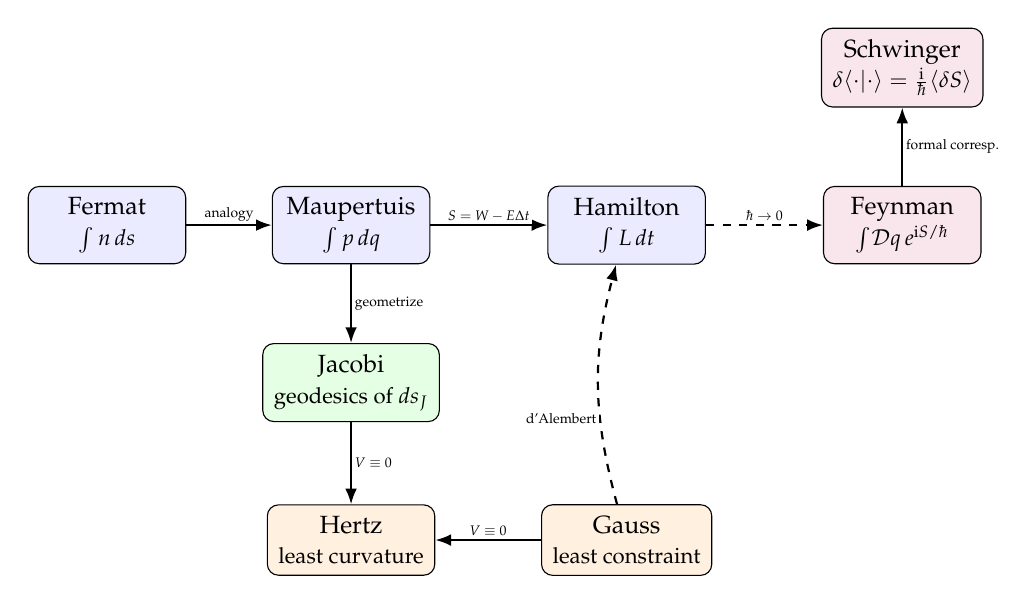
\begin{tikzpicture}[
  box/.style={draw, rounded corners, align=center, minimum height=8mm, minimum width=20mm, inner sep=4pt, font=\small},
  classint/.style={box, fill=blue!8},
  classgeo/.style={box, fill=green!10},
  classdiff/.style={box, fill=orange!12},
  quant/.style={box, fill=purple!10},
  arr/.style={-{Latex[length=2mm]}, thick},
  darr/.style={arr, dashed},
  lbl/.style={font=\tiny, fill=white, inner sep=1pt}
]
  \node[classint] (fermat) at (0,0) {Fermat\\ \footnotesize $\int n\,ds$};
  \node[classint] (maupertuis) at (3.1,0) {Maupertuis\\ \footnotesize $\int p\,dq$};
  \node[classint] (hamilton) at (6.6,0) {Hamilton\\ \footnotesize $\int L\,dt$};
  \node[quant] (feynman) at (10.1,0) {Feynman\\ \footnotesize $\int\! \mathcal D q\, e^{\ii S/\hbar}$};
  \node[quant] (schwinger) at (10.1,2.0) {Schwinger\\ \footnotesize $\delta\langle\cdot|\cdot\rangle=\tfrac{\ii}{\hbar}\langle\delta S\rangle$};

  \node[classgeo] (jacobi) at (3.1,-2.0) {Jacobi\\ \footnotesize geodesics of $ds_J$};
  \node[classdiff] (hertz) at (3.1,-4.0) {Hertz\\ \footnotesize least curvature};
  \node[classdiff] (gauss) at (6.6,-4.0) {Gauss\\ \footnotesize least constraint};

  \draw[arr] (fermat) -- node[lbl,above]{analogy} (maupertuis);
  \draw[arr] (maupertuis) -- node[lbl,above]{$S=W-E\Delta t$} (hamilton);
  \draw[darr] (hamilton) -- node[lbl,above]{$\hbar\to0$} (feynman);
  \draw[arr] (feynman) -- node[lbl,right]{formal corresp.} (schwinger);
  \draw[arr] (maupertuis) -- node[lbl,right]{geometrize} (jacobi);
  \draw[arr] (jacobi) -- node[lbl,right]{$V\equiv 0$} (hertz);
  \draw[arr] (gauss) -- node[lbl,above]{$V\equiv0$} (hertz);
  \draw[darr] (gauss) to[bend left=15] node[lbl,pos=0.35,left]{d'Alembert} (hamilton);
\end{tikzpicture}
\caption{The variational atlas. Solid arrows are exact derivations (Sections~\ref{sec:hamilton}--\ref{sec:schwinger}); the dashed arrow from Hamilton to Feynman is the $\hbar\to0$ stationary-phase limit, and from Gauss to Hamilton is the classical (non-constrained) reduction via d'Alembert's principle -- asymptotic/formal correspondences, not identities.}
\label{fig:atlas}
\end{figure}

\section{Extension to fields}

Everything above generalizes, with $q^i(t)$ replaced by a field $\varphi^a(x)$ on spacetime, by promoting Hamilton's principle to
\[
\delta\!\int L(\varphi,\partial_\mu\varphi)\,d^4x=0,
\]
giving the field Euler--Lagrange equations
\[
\partial_\mu\!\left(\frac{\partial L}{\partial(\partial_\mu\varphi^a)}\right) = \frac{\partial L}{\partial\varphi^a}.
\]
The Hamilton/Maupertuis distinction --- which coordinate plays the role of ``time'' to be fixed versus freed --- becomes, in field theory, the question of treating one spacetime direction asymmetrically (ordinary Hamiltonian field theory) versus all of them symmetrically (the De Donder--Weyl covariant Hamiltonian formalism and multiple-integral calculus of variations, treated as their own chapter of this book). Gauss's and Hertz's differential principles do not obviously survive the passage to fields in a useful form, which is itself worth noting: instantaneous, finite-dimensional least-constraint reasoning does not have an established infinite-dimensional counterpart of comparable power.

\section{Equations of motion are primary; variational principles are heuristics}
\label{sec:primacy}

None of the principles in this chapter is more ``true'' than the others in the sense of better describing the real-world trajectory: for a holonomic, energy-conserving system they are jointly compatible, and physically indistinguishable in their predictions. What differs is which real-world question each idealization is built to answer directly. ``What configuration is the system in at time $t$?'' is answered most directly by Hamilton's principle. ``What is the geometric shape of the orbit, independent of how fast it is traversed?'' is answered most directly by Maupertuis' and Jacobi's. ``What happens to constraint forces at this instant?'' is Gauss's question. ``What are the possible outcomes of a measurement, and with what amplitude?'' is Schwinger's and Feynman's. Section~\ref{sec:nonequivalence} was the cautionary half of that remark: the compatibility just described holds trajectory by trajectory, not problem by problem.

Put the two observations together and a sharper claim follows, and this chapter is the argument for it.

\begin{motto}
\textbf{Thesis.} The equations of motion are the real-world content of a mechanical theory: the differential, causal, initial-value statement that is actually checked against experiment and that alone stays invariant across every reformulation in this chapter. A variational principle is an ideal-world heuristic for \emph{finding} those equations --- a scaffold engineered so that stationarity reproduces a differential law already fixed by other means. It is not itself a law of nature, and no metaphysical content should be read into the word ``least.''
\end{motto}

\begin{remark}[underdetermination]
Table~\ref{tab:summary} lists objects varied of genuinely different mathematical kinds --- a time integral ($S$), a curve integral ($W$), a pointwise quadratic form ($Z(\ddot q)$), an operator matrix element --- all of which are stationary exactly on the solutions of the same equations of motion. If any one of these were the law nature ``obeys,'' the others would need explaining away; there is no principled way to prefer $\int L\,dt$ over $Z(\ddot q)$ as the fundamental fact and demote the other to derived curiosity. What is invariant across all of them, and hence what deserves to be called primary, is the one thing they all agree on: the equations of motion themselves.
\end{remark}

\begin{remark}[Gauss and Hertz remove the teleology]
A global, fixed-endpoint statement like Hamilton's principle can sound as though the system ``surveys'' every possible history between two moments before choosing the actual one --- historically the most seductive (and most criticized) reading of least action. Gauss's principle removes this appearance entirely: Proposition~\ref{prop:gauss-dalembert} showed it equivalent, instant by instant, to $(m_a\ddot{\vec r}_a-\vec F_a)\cdot\delta\vec r_a=0$, i.e.\ to Newton's second law together with d'Alembert's principle, with no reference to the future or to any global comparison of histories. The same content that Hamilton's principle packages as ``compare the whole path'' is available, undiminished, as a purely local, instant-by-instant fact. Hertz's principle (Section~\ref{sec:hertz}) is the same point in geometric dress: force-free motion is just the straightest available path, an entirely local notion of curvature. Nothing about the physics requires the global packaging; the global packaging is a choice of heuristic, not a discovery about how nature decides.
\end{remark}

\begin{remark}[fragility shows the direction of justification]
Remark~\ref{rem:fragility} is the clearest evidence for which way the inference actually runs. Naively extremizing $\int L\,dt$ under a nonholonomic constraint gives the \emph{wrong} equations of motion (the vakonomic ones); the \emph{right} equations (Lagrange--d'Alembert) are fixed independently, by direct mechanical reasoning about constraint forces and virtual work, and it is against that independently-known target that the naive variational guess is judged and rejected. Section~\ref{sec:gauss} was accepted as ``the right principle'' \emph{because} it reproduces the equations of motion known to be correct on other grounds --- not the other way around. If a variational principle were itself the primary law, it would never need to be repaired against a differential equation assumed to be more trustworthy than it is.
\end{remark}

\begin{remark}[the equations of motion are the robust object]
Section~\ref{sec:nonequivalence} showed that once a potential has several minima, the variational \emph{problem} can fragment: the textbook Maupertuis competition can have an empty domain, the Generalized Maupertuis Principle's competition can fail to contain an extremal, and brake-orbit multiplicity can make ``the'' fixed-energy solution ambiguous. Through all of this the equation of motion itself --- an ordinary differential equation with a well-posed initial-value problem --- never fragments, never loses a solution, and never multiplies one; it is exactly as well behaved for ten wells as for one. The variational reformulation is the fragile, construction-dependent object; the differential law is the robust one.
\end{remark}

\begin{remark}[even ``derived versus assumed'' is bookkeeping]
Section~\ref{sec:schwinger-classical} made a further, sharper version of the same point at the classical level: whether $\dot q^i=\partial H/\partial p_i$ counts as a consequence of a variational principle or as a definition adopted before any variation is taken depends entirely on whether one varies $q$ alone (ordinary Hamilton's principle) or $q$ and $p$ independently (the phase-space principle). The two canonical equations themselves do not change; only the bookkeeping of which one gets called ``derived'' does. A fact about nature should not depend on which variational scaffold was used to reach it.
\end{remark}

\begin{remark}[the name itself overclaims]
Even calling these ``least'' action is often simply false. Once a trajectory passes a conjugate point --- exactly where the curvature of the Jacobi metric of Section~\ref{sec:jacobi} turns the second variation indefinite --- the stationary trajectory is a \emph{saddle} of $S$, not a minimum. Hamilton himself never claimed a minimum principle, only a stationary one; ``least action'' is a historical label surviving from a reading the mathematics does not support in general.
\end{remark}

The historical record backs this reading of the founders' own intentions, not merely a modern gloss on them. Maupertuis' 1746 memoir was titled, without irony, ``the laws of motion and of rest deduced from a metaphysical principle'' --- he offered least action as evidence of a providential economy in nature, not as a mathematical convenience. But d'Alembert, Lagrange, Hertz and Jacobi --- three of whom are principal subjects of this very chapter --- explicitly rejected any ontological economy-of-nature behind their own principles, treating least action as what Panza and Goldstine call a figurative scientific model rather than a metaphysical discovery. Mach's \emph{Science of Mechanics} (1883) makes the case most sharply, in a chapter pointedly titled \emph{Theological, Animistic, and Mystical Points of View in Mechanics}, followed immediately by one titled \emph{The Economy of Science}: for Mach, least-action-type statements are \emph{theorems} --- consequences, economically redescribing what is already contained in Newton's laws --- not \emph{principles} in the sense of directly-intuited primitive facts (his examples of genuine principles are the lever and virtual displacements). Their teleological gloss, Mach argued, was a product of a theologically-tempered era, not a discovery about how nature operates. Helmholtz, writing in the same period, offered the more constructive half of the same demotion: whatever their metaphysical status, least-action-type statements had proved, again and again, a powerful heuristic and leitmotif for finding the governing equations of new domains of physics before those equations were otherwise known --- exactly the role this book assigns them, and exactly why this chapter surveys so many of them side by side rather than picking one as ``the'' principle.

This chapter's own atlas (Figure~\ref{fig:atlas}) is therefore a small instance of the book's larger cartographic thesis: many overlapping charts, no chart mistaken for the territory. The equations of motion are the territory; Hamilton's, Maupertuis', Gauss's, Hertz's and Schwinger's principles are charts of it, each drawn to make some feature --- boundary-value structure, orbit shape, instantaneous constraint forces, geodesic curvature, operator structure --- easy to read off, at the cost of making others (as Section~\ref{sec:nonequivalence} showed) harder to see or entirely invisible. Mistaking a chart, however elegant or historically freighted, for the territory is exactly the real-world/ideal-world category error this book exists to name. (The fragility of the least-action reading in particular is developed at greater length in the companion paper on that subject.)

\begin{reflectionbox}
\textbf{Reflection questions.}
\begin{enumerate}[itemsep=2pt]
\item Why does Gauss's principle handle nonholonomic constraints correctly while a naive fixed-endpoint application of Hamilton's principle does not? Locate exactly where the two constructions part ways.
\item Proposition~\ref{prop:S-W} shows $S=W-E\Delta t$ along a trajectory. Is this an identity for \emph{any} curve of energy $E$, or only along the true trajectory? What changes if the trial curve does not conserve $E$ pointwise?
\item Construct the Jacobi metric for the Kepler problem, $V(r)=-k/r$. For which range of energies $E$ is the Jacobi metric's curvature everywhere negative, and what does this imply about neighboring orbits?
\item Schwinger's action $S$ is, like Hamilton's, a time integral, yet the action principle built on it is called differential. In what precise sense is it differential, and what would it mean for a variational principle to be differential in a stronger sense than Schwinger's?
\item Hertz's principle presupposes holonomic constraints. Sketch what goes wrong if one tries to apply ``least curvature in configuration space'' directly to a nonholonomically constrained system, and relate the failure to Section~\ref{sec:gauss}.
\item Why does fixing the \emph{pointwise} energy $E$ on trial curves (Definition~\ref{def:maupertuis-old}) leave almost no freedom to vary a one-dimensional trial trajectory, while fixing only the \emph{mean} energy $\bar E$ (Section~\ref{sec:reciprocal}) does not? Work through the free-particle-on-a-segment example.
\item In the classical phase-space principle of Section~\ref{sec:schwinger-classical}, $\delta p_i$ is left unconstrained at the endpoints while $\delta q^i$ is not. What would go wrong --- which equation would fail to be derivable --- if both were required to vanish at $t_1$ and $t_2$?
\item For a double-well potential with barrier height $V_b$, sketch $E(T)$ for a Hamilton-principle trajectory that crosses the barrier, and $T(E)$ for the corresponding Maupertuis/GMP trajectory. Why must both curves stay confined to $E>V_b$, and which of the two formulations makes that restriction obvious from the setup alone, rather than only from the solution?
\item Section~\ref{sec:primacy} argues that a variational principle earns its keep by reproducing an independently-known equation of motion, not the reverse. Is there a case in this chapter where the direction of justification genuinely runs the other way --- where a variational principle revealed an equation of motion (or a symmetry) that was not already known on other grounds? What would that require of the argument?
\item Set $\gamma=0$ in the Herglotz example. Confirm the generalized Euler--Lagrange equation reduces to the ordinary one, and explain why $\partial L/\partial z$ is exactly what has to vanish for that reduction --- relate this to the remark that Herglotz's principle reduces to Hamilton's when $L$ does not depend on $z$.
\item Marinov's phase-space path integral leaves $p$ free at both endpoints while Feynman's configuration-space path integral fixes $q$ at both endpoints and never mentions $p$'s boundary values at all. Where, physically, does the momentum-space information ``go'' in Feynman's version, and why does it have to reappear as a free integration in Marinov's?
\item Marinov's phase action explains the multivaluedness of Hamilton's principal function $\mathcal A$ as an artifact of a Legendre transform applied to a single-valued function $\Phi$. Hamilton's principal function is itself obtained from $\Phi$ by fixing the two separate endpoints rather than their midpoint. Is there an analogous Legendre-transform explanation for the multiplicity of Maupertuis/GMP solutions in Section~\ref{sec:nonequivalence}, or does that multiplicity have a different source?
\end{enumerate}
\end{reflectionbox}

\section*{Bibliography}
\begin{enumerate}[label={[\arabic*]}, itemsep=1pt]
\item W.~R.~Hamilton, ``On a General Method in Dynamics,'' \emph{Phil.\ Trans.\ R.\ Soc.} (1834); ``Second Essay on a General Method in Dynamics,'' \emph{Phil.\ Trans.\ R.\ Soc.} (1835).
\item P.~L.~M.~de Maupertuis, ``Accord de différentes lois de la nature qui avaient jusqu'ici paru incompatibles,'' \emph{Mém.\ Acad.\ Sci.\ Paris} (1744); ``Les loix du mouvement et du repos déduites d'un principe métaphysique,'' \emph{Hist.\ Acad.\ Roy.\ Sci.\ Belles-Lettres, Berlin} (1746).
\item L.~Euler, \emph{Methodus inveniendi lineas curvas maximi minimive proprietate gaudentes}, Additamentum II (1744).
\item C.~G.~J.~Jacobi, \emph{Vorlesungen über Dynamik}, ed.\ A.~Clebsch (1866; lectures of 1842--43).
\item H.~Seifert, ``Periodische Bewegungen mechanischer Systeme,'' \emph{Math.\ Z.} \textbf{51}, 197 (1948).
\item R.~Giambò, F.~Giannoni and P.~Piccione, ``Multiple Orthogonal Geodesic Chords and a Proof of Seifert's Conjecture on Brake Orbits'' [arXiv:2002.09687]; ``Potential Wells with a Unique Brake Orbit: Counterexamples to a Conjecture by H.~Seifert'' [arXiv:1203.5198].
\item C.~F.~Gauss, ``Über ein neues allgemeines Grundgesetz der Mechanik,'' \emph{J.\ Reine Angew.\ Math.} \textbf{4} (1829).
\item J.~W.~Gibbs, ``On the Fundamental Formulae of Dynamics,'' \emph{Am.\ J.\ Math.} \textbf{2}, 49 (1879); P.~Appell, ``Sur une forme générale des équations de la dynamique,'' \emph{J.\ Reine Angew.\ Math.} \textbf{121}, 310 (1900).
\item G.~Herglotz, unpublished lectures, Göttingen (1930); B.~Georgieva and R.~Guenther, ``First Noether-Type Theorem for the Generalized Variational Principle of Herglotz,'' \emph{Topol.\ Methods Nonlinear Anal.} \textbf{20}, 261 (2002); A.~Bravetti, H.~Cruz and D.~Tapias, ``Contact Hamiltonian Mechanics,'' \emph{Ann.\ Phys.} \textbf{376}, 17 (2017).
\item E.~Mach, \emph{Die Mechanik in ihrer Entwicklung historisch-kritisch dargestellt} (1883); trans.\ \emph{The Science of Mechanics}, ch.~IV, \S\S II, IV (``Theological, Animistic, and Mystical Points of View in Mechanics''; ``The Economy of Science'').
\item H.~Hertz, \emph{Die Prinzipien der Mechanik in neuem Zusammenhange dargestellt} (1894).
\item C.~G.~Gray, G.~Karl and V.~A.~Novikov, ``Progress in Classical and Quantum Variational Principles,'' \emph{Rep.\ Prog.\ Phys.} \textbf{67}, 159 (2004) [arXiv:physics/0312071].
\item G.~Karl and V.~A.~Novikov, ``New Variational Principles in Classical and Semiclassical Mechanics,'' in the Michael Marinov Memorial Volume, \emph{Multiple Facets of Quantization and Supersymmetry}, eds.\ M.~Olshanetsky and A.~Vainshtein (World Scientific, 2002) [arXiv:hep-ph/0112349].
\item É.~Cartan, \emph{Leçons sur les invariants intégraux} (Hermann, Paris, 1922).
\item P.~Weiss, ``On the New Field Theory,'' \emph{Proc.\ R.\ Soc.\ Lond.\ A} \textbf{159}, 355 (1936); ``On the Hamilton--Jacobi Theory and Quantization of a Dynamical Continuum,'' \emph{Proc.\ R.\ Soc.\ Lond.\ A} \textbf{169}, 102 (1938).
\item P.~de Fermat, letter to Cureau de la Chambre (1662).
\item J.~Schwinger, ``The Theory of Quantized Fields I,'' \emph{Phys.\ Rev.} \textbf{82}, 914 (1951).
\item M.~S.~Marinov, ``Path Integrals in Quantum Theory: An Outlook of Basic Concepts,'' \emph{Phys.\ Rep.} \textbf{60}, 1 (1980); ``An Alternative to the Hamilton--Jacobi Approach in Classical Mechanics,'' \emph{J.\ Phys.\ A: Math.\ Gen.} \textbf{12}, 31 (1979).
\item R.~P.~Feynman, ``Space-Time Approach to Non-Relativistic Quantum Mechanics,'' \emph{Rev.\ Mod.\ Phys.} \textbf{20}, 367 (1948).
\item C.~Lanczos, \emph{The Variational Principles of Mechanics}, 4th ed.\ (1970).
\item W.~Yourgrau and S.~Mandelstam, \emph{Variational Principles in Dynamics and Quantum Theory}, 3rd ed.\ (1968).
\item V.~I.~Arnold, \emph{Mathematical Methods of Classical Mechanics} (1989).
\item E.~T.~Whittaker, \emph{A Treatise on the Analytical Dynamics of Particles and Rigid Bodies}, 4th ed.\ (1937).
\end{enumerate}

\end{document}
